Here we outline the details regarding the energy based model training. Given an EBM of the form,
\begin{equation}
    p_\theta(x)=\frac{1}{C_\theta}e^{-E(\theta,x)},\qquad C_\theta=\int e^{-E(\theta,x)}dx,
\end{equation}
we consider the diffusion limit of the PCD algorithm given in \cite{oliva2025uniformintimeconvergenceboundspersistent} and adapt the system of equations for under-damped Langevin dynamics. After approximating the expectation $\mathbb{E}_{X\sim p_\theta}[\nabla_\theta E(\theta,X)]$ in the exact maximum likelihood gradient, we have the particle approximation,
\begin{equation*}
    \nabla_\theta\ell\approx-\frac{1}{N}\sum_{n=1}^N\nabla_\theta E(\theta,X^n)+\frac{1}{M}\sum_{m=1}^M\nabla_\theta E(\theta, y^m),
\end{equation*}
with particles $\{X^i\}_{i=1}^N$ and fixed data $\{y^m\}_{m=1}^M$. In our framework, this may be written with
\begin{equation*}
    F(\theta,X^{i})=-\nabla_\theta E(\theta,X^i)+\frac{1}{M}\sum_{m=1}^M\nabla_\theta E(\theta, y^m).
\end{equation*}
We parametrise the energy function used for training in the 2D synthetic datasets experiments with a 3 hidden-layer, 128-unit \textit{SiLU} network. Throughout training we assume $C_\theta<\infty$ such that the model is a valid density for every parameter value we visit. We pick three different synthetic datasets to train on. Each has closed form density functions and are described below,

\textbf{Rings}. We consider two concentric rings with different radii but sharing the same total densities along their circumferences. In polar coordinates we define the independent distributions,
\begin{equation*}
    p_r(r)=\frac{1}{2}\mathcal{N}_{\mathrm{tr}}(r;r_1,\sigma^2,[0,\infty))+\frac{1}{2}\mathcal{N}_{\mathrm{tr}}(r;r_2,\sigma^2,[0,\infty)),\qquad r\ge 0.
\end{equation*}
where $\mathcal{N}_{\mathrm{tr}}(\cdot\,;\mu,\sigma,[0,\infty))$ is a truncated Gaussian with support on the non-negative reals $[0,\infty)$. Independently draw $A\sim\textrm{Uniform}(0,2\pi)$ and set $\mathbf{x}=r(\cos A,\sin A)$. The \textit{rings} distribution is exactly the Cartesian parametrisation,
\begin{equation*}
    p(\mathbf{x})=\frac{1}{4\pi\Vert\mathbf{x}\Vert}\left(\mathcal{N}_{\mathrm{tr}}(\|x\|;r_1,\sigma^2,[0,\infty))+\mathcal{N}_{\mathrm{tr}}(\|x\|;r_2,\sigma^2,[0,\infty))\right).
\end{equation*}
We note for large enough $r_1,r_2$ and small enough $\sigma$, the truncation effects are negligible and we may simply write the distributions with regular Gaussians, giving us closed-form expressions for the score. Here, we take $r_1=1,r_2=2.5$ and $\sigma=0.2$.

\textbf{Beads}. We consider a mixture of isotropic Gaussians centred equiradially from the origin. For $n$ Gaussians we define the density,
\begin{equation*}
    p(\mathbf{x})=\frac{1}{n}\sum_{k=1}^n\mathcal{N}(\mathbf{x}; l_k,\sigma^2)
\end{equation*}
with $l_k=(\sin(2\pi k/n),\cos(2\pi k/n))$. Here we take $n=5$ and $\sigma=0.1$.

\textbf{Lattice}. We consider a mixture of isotropic Gaussians centred on the points of a $n\times n$ lattice. Denoting these points $m_k=(\lfloor k/n\rfloor-(n-1)/2,k-n\lfloor k/n\rfloor-(n-1)/2)$ for $k=0,...,n^2-1$ we have the density,
\begin{equation*}
    p(\mathbf{x})=\frac{1}{n^2}\sum_{k=0}^{n^2-1}\mathcal{N}(\mathbf{x};\alpha m_k,\sigma^2),
\end{equation*}
where $\alpha$ is some scaling parameter. We take $n=3$ and $\alpha=\sqrt{2}$ and 
$\sigma=\sqrt{2}/10$. These distributions can be sampled from exactly with built-in functions to create training datasets. We generate 10,000 samples for each dataset.

To train the 2D synthetic datasets, we compare the different methods below,
\begin{itemize}
    \item \gls*{pcd} - We implement persistent contrastive divergence as a baseline. Particles are updated with a ULA kernel step, whilst parameters are updated with gradient descent.
    \item \gls*{mmfpo} - We accelerate by updating particles and parameters with under-damped Langevin using our proposed discretisation.
\end{itemize}
For each method we use a set of $10,000$ particles, matching the number of data-points, all initialised from i.i.d standard Gaussians. For \gls*{mmfpo}, we initialise particle momenta from i.i.d standard Gaussians and initialise parameter momenta with zeros.

For the performance metric, we estimate the Fisher divergence as it does not require computing the normalising constant of the learnt energy and we have access to the score of the data distribution. We compute the empirical Fisher divergence at each iteration with $M_{\mathrm{eval}}=10,000$ samples from the data distribution,
\begin{equation*}
    \widehat D_{\mathrm F}(\theta)
    =\frac1{2M_{\mathrm{eval}}}
    \sum_{m=1}^{M_{\mathrm{eval}}}
    \left\|
    \nabla_x\log p_{\mathrm{data}}(z^m)
    +\nabla_xE(\theta,z^m)
    \right\|^2,
    \qquad
    z^m\sim p_{\mathrm{data}}.
\end{equation*}
If the model family contains $p_{\mathrm{data}}$ and the usual score-identifiability and integrability conditions hold, the Fisher divergence shares the same zero at $p_\theta=p_{\mathrm{data}}$ with $\mathrm{KL}(p_{\mathrm{data}}\|p_\theta)$. Note that for the \textit{rings} dataset, whilst the score diverges at zero, the empirical calculation evaluates scores at samples from the data distribution which are sufficiently far from zero with high probability. We do not claim that their minimisers coincide under model misspecification or that the minimising neural-network parameter is unique.

We keep a fixed computational budget for each method, which for us is equivalent to a fixed number of training iterations since each iteration uses the same number of energy evaluations and gradient evaluations. We begin training with a shared step-size between parameter and particle updates for both \gls*{pcd} and \gls*{mmfpo}. In practice the oscillatory nature of the underdamped dynamics in \gls*{mmfpo} result in greater training fluctuations. So we also design learning rate decay schedules on the parameter step-sizes that decrease over iterations. In particular for the \textit{lattice} dataset, we use the linear decay,

\begin{equation}
    \text{lr}(t)=\begin{cases}
        h_0 & t\le L, \\
        h_0\left(\frac{T-t}{T-L}\right)+h_T\left(\frac{t-L}{T-L}\right) & L<t<T, \\
        h_T & t\ge T,
    \end{cases}
\end{equation}
where $h_0,h_T$ are hyperparameters starting and ending step-sizes, $L,T$ are times we pick to decay between. In general these are all hyperparameters but with the goal of damping the training fluctuations, extensive tuning is not required. 
For the \textit{lattice} dataset, we take $T=400,000$ to be the fixed number of training iterations, $L=6000$ and $h_T=h_0/10$. For the \textit{rings} and \textit{beads} datasets we do not use any scheduler and run for $T=150,000$ iterations. We run the training 25 times on different seeds and report the average Fisher divergence with standard-deviation error envelopes across iterations. All models were trained and evaluated on a high-performance computing cluster provided by the institution. Training was done on a NVIDIA RTX 6000 Ada Generation GPU with 18176 cores and 48GB of on-GPU memory. We plot the learnt probability densities and freshly generated samples in Figure~\ref{fig:models}.

\begin{figure*}[ht]
\begin{minipage}[t]{0.32\textwidth}
        \centering
        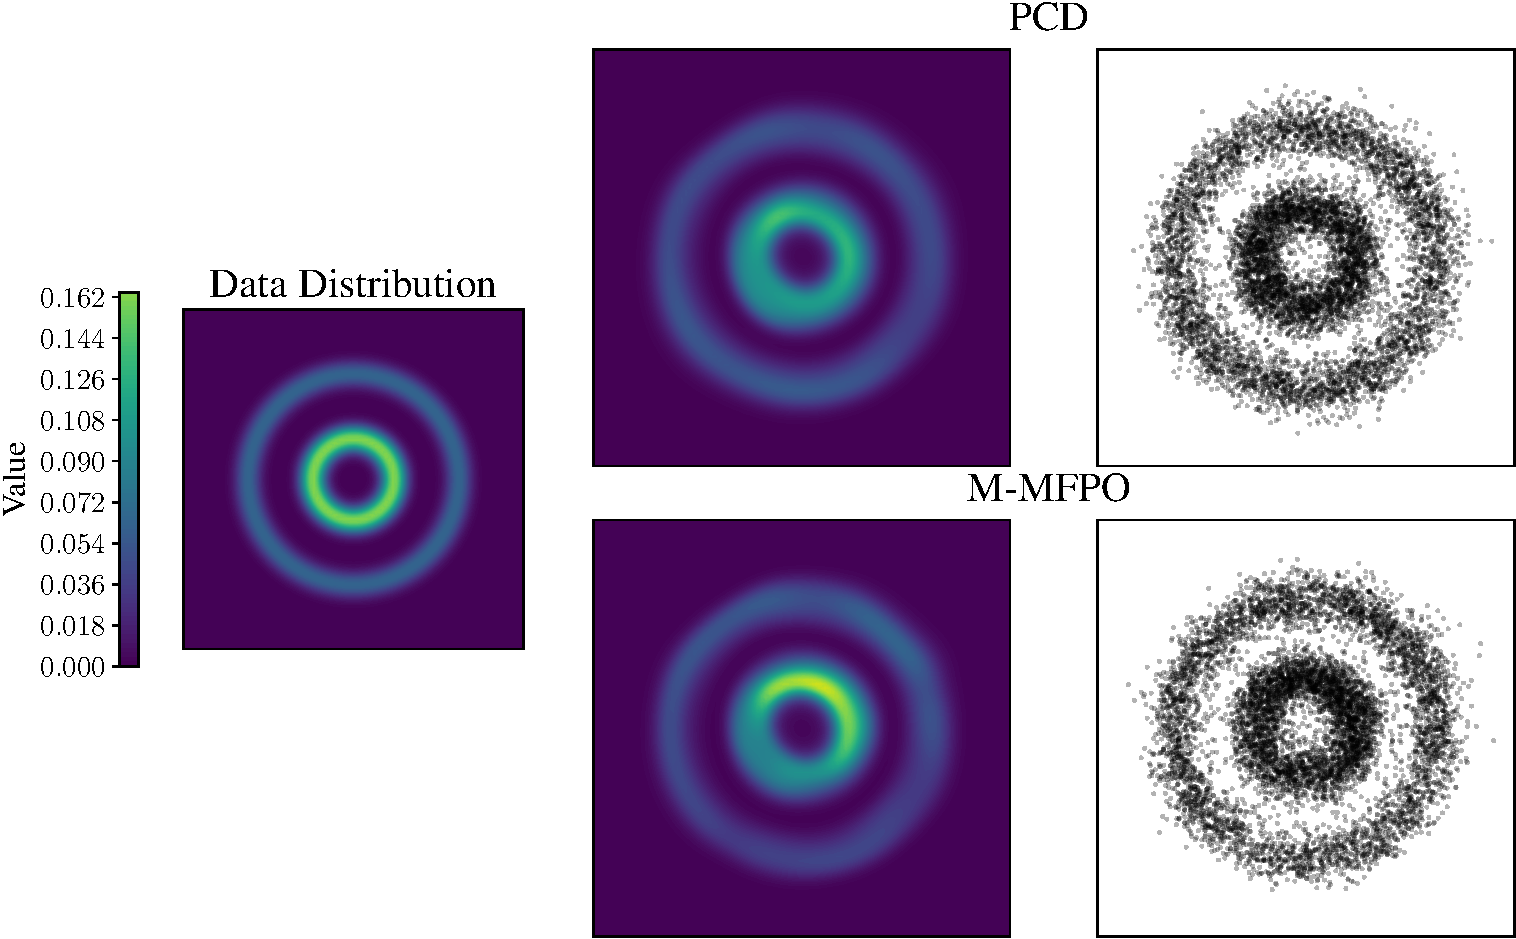
\includegraphics[width=\textwidth]{images/main/final_rings_models.pdf}
    \end{minipage}
    \hfill
    \begin{minipage}[t]{0.32\textwidth}
        \centering
        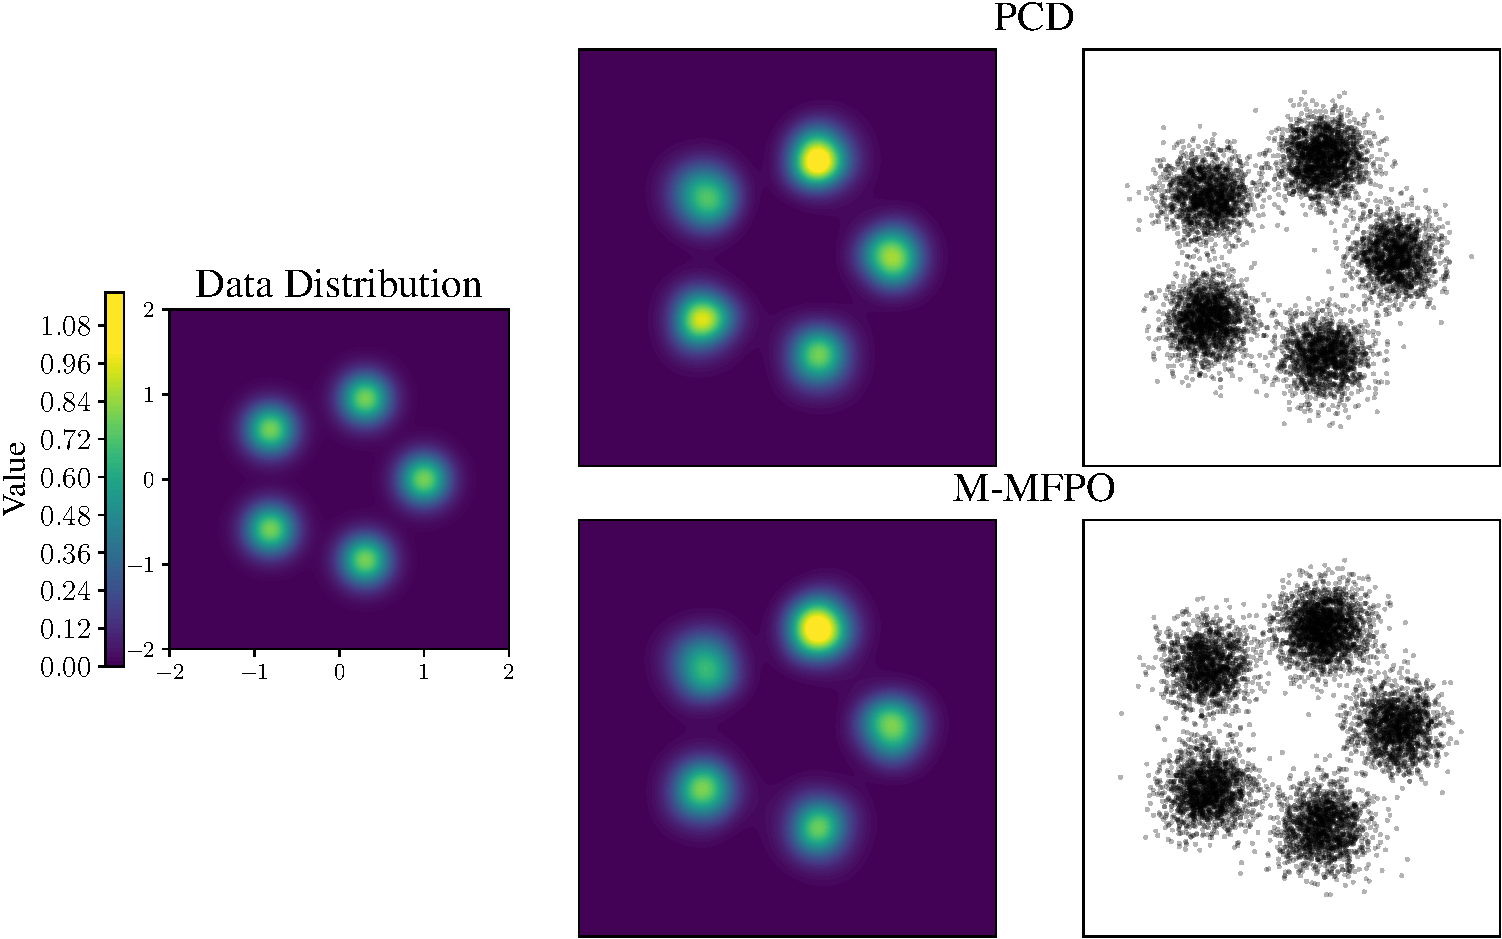
\includegraphics[width=\textwidth]{images/main/final_beads_models.pdf}
    \end{minipage}
    \hfill
    \begin{minipage}[t]{0.32\textwidth}
        \centering
        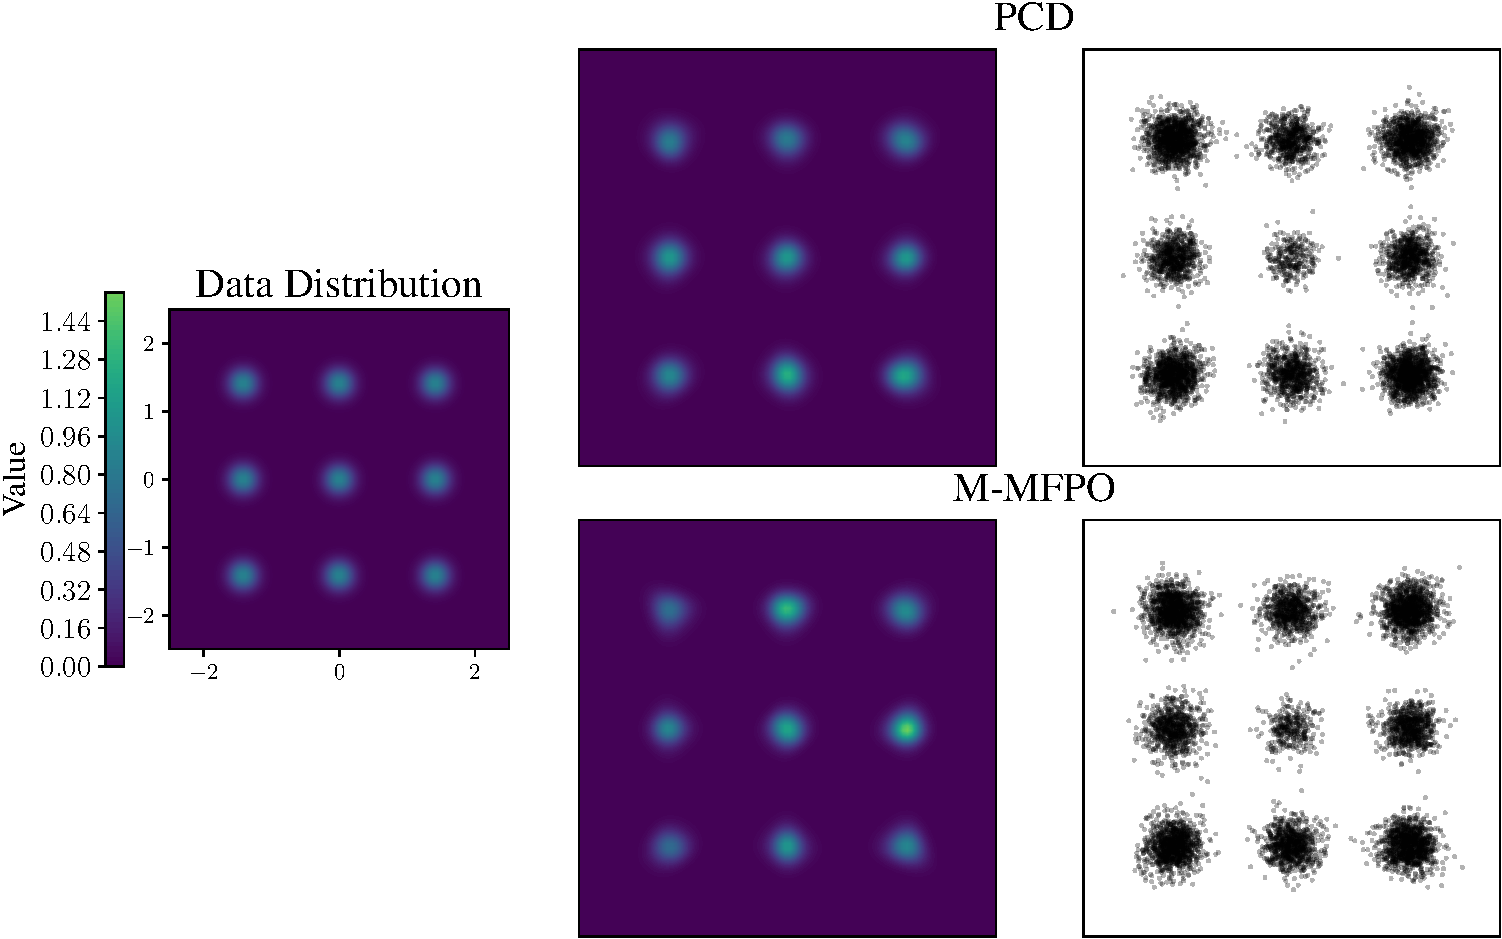
\includegraphics[width=\textwidth]{images/main/final_lattice_models.pdf}
    \end{minipage}
    \caption{Comparison of learnt densities and fresh samples from the model for the \textit{rings} dataset (left), \textit{beads} dataset (middle), and \textit{lattice} dataset (right).}
    \label{fig:models}
\end{figure*}

For the baseline \gls*{pcd} method, we only have step-size as a hyperparameter, whilst for \gls*{mmfpo} we have both step-size and friction. When tuning, there is a trade-off between speed and accuracy, with smaller step-sizes typically yielding a lower Fisher divergence at the cost of slower convergence. We plot in Figures \ref{fig:od_beads_hps} and \ref{fig:obabo_beads_hps} the effects of hyperparameters for training the \textit{beads} dataset on both the speed of convergence, which we measure with the area under the curve ($AOC$) and the accuracy at the end of training, which we measure by an averaged final Fisher divergence ($FD_\infty$). We record the Fisher divergence every 100 iterations over 100,000 iterations and evaluate the $AOC$ as the sum and $FD_\infty$ as the average of the last 20 recordings. We seek the hyperparameters producing both the lowest $AOC$ and $FD_\infty$.
\begin{figure}[h]
    \centering
    \begin{minipage}[b]{0.48\textwidth}
        \centering
        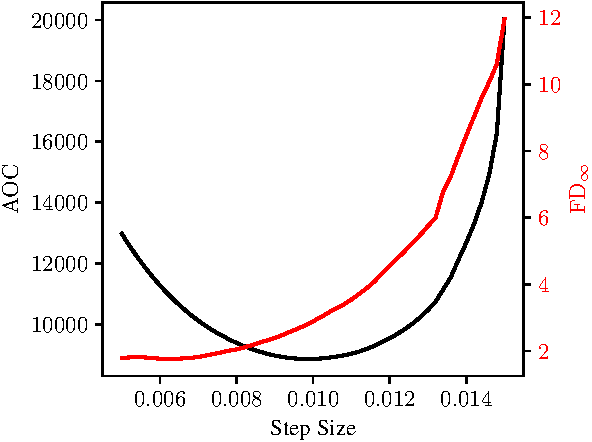
\includegraphics[width=0.75\textwidth]{images/appendix/fd_summary_beads_od_hps.pdf}
    \end{minipage}
    \hfill
    \begin{minipage}[b]{0.48\textwidth}
        \centering
        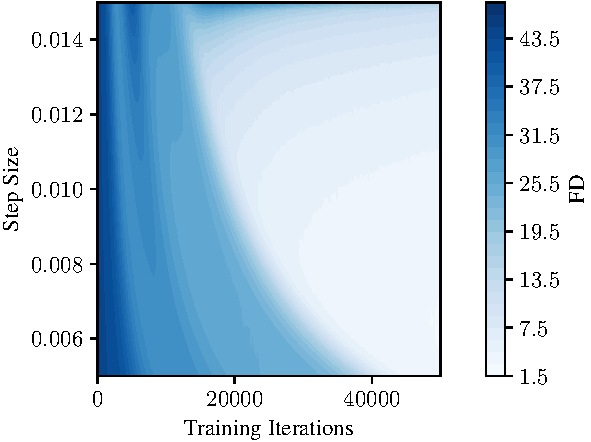
\includegraphics[width=0.75\textwidth]{images/appendix/fd_heatmap_beads_od_hps.pdf}
    \end{minipage}
    \caption{Effect of step-size on convergence ($AOC$) and converged-value ($FD_\infty$) for PCD (left) and contour plot of Fisher divergence across iterations for a range of step-sizes (right)}
    \label{fig:od_beads_hps}
\end{figure}

We see in Figure~\ref{fig:od_beads_hps} increasing step-size leads to a worse convergence and decreasing step-size leads to much slower convergence. There is a minor trade off between the $AOC$ and $FD_\infty$ if both are to be minimised and we take the step-size $h=0.01$ in the final comparison.
\begin{figure}[htbp]
    \centering
    \begin{minipage}[b]{0.48\textwidth}
        \centering
        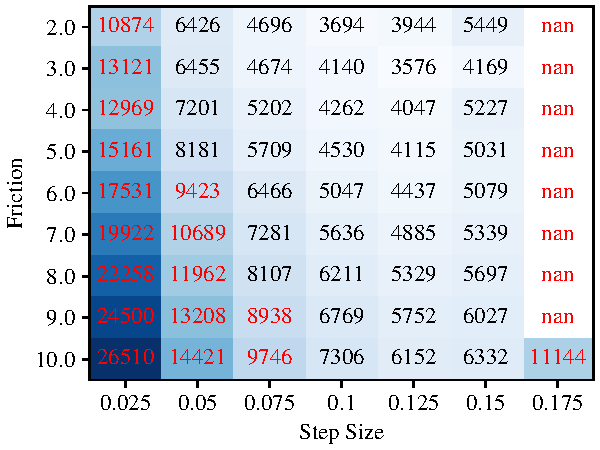
\includegraphics[width=0.75\textwidth]{images/appendix/beads_obabo_aoc_heatmap.pdf}
    \end{minipage}
    \hfill
    \begin{minipage}[b]{0.48\textwidth}
        \centering
        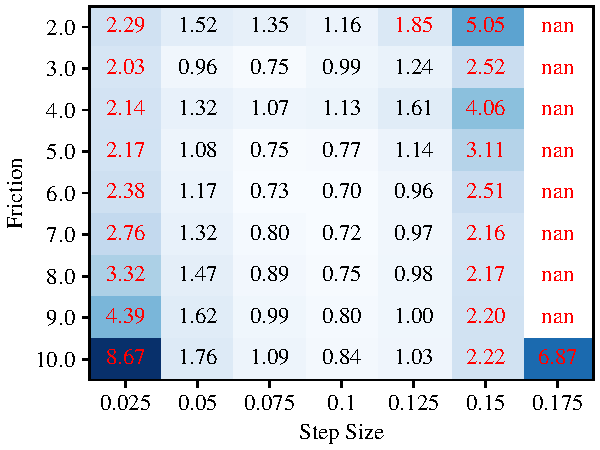
\includegraphics[width=0.75\textwidth]{images/appendix/beads_obabo_l_inf_heatmap.pdf}
    \end{minipage}
    \caption{Effect of step-size and friction on the $AOC$ (left) and $FD_\infty$ (right). Values in black are lower than the lowest observed corresponding value in the overdamped PCD across all step-sizes (lower is better).}
    \label{fig:obabo_beads_hps}
\end{figure}
We pick optimal hyperparameters for both methods from the sweeps whilst also ensuring long-term stability of the training. These are summarised in table~\ref{tab:ebm_training_hps}. Note that from Figure~\ref{fig:obabo_beads_hps}, values in black beat the best \gls*{pcd} hyperparameters and we see there are particular choices of friction and step-size that yield an $AOC$ and $FD_\infty$ that are both better than the best corresponding \gls*{pcd} hyperparameter.
\begin{table}[h]
    \caption{List of hyperparameters used in the 2D \gls*{ebm} training experiments for \gls*{pcd} and \gls*{mmfpo} methods across different datasets. Note that we use a linear step-size schedule for the \textit{lattice} dataset and the displayed step-size is the initial step-size.}
    \label{tab:ebm_training_hps}
    \centering
    \setlength{\tabcolsep}{2pt}
    {\begin{tabular}{l@{\hspace{24pt}}c@{\hspace{24pt}}cc}
        \toprule
        \multirow{2}{*}{Dataset} & \multicolumn{1}{c}{\gls*{pcd}} & \multicolumn{2}{c}{\gls*{mmfpo}} \\
        \cmidrule(lr){2-2}\cmidrule(lr){3-4}
        & \makecell{(initial) step-size} & \makecell{step-size} & \makecell{friction} \\
        \midrule
        \textbf{rings} & 
        0.016 & 
        0.19 & 
        5.5 \\
        \textbf{beads} & 
        0.01 & 
        0.1 & 
        6.0 \\
        \textbf{lattice} & 
        0.004 & 
        0.075 & 
        8.0 \\
        \bottomrule
    \end{tabular}}
\end{table}